\documentclass[twocolumn]{article}
\usepackage[utf8]{inputenc}

\title{Beautiful Empathy}
%\date{December 2020}

% \usepackage{natbib}
\usepackage{graphicx}
\usepackage{amsmath}
\newcommand{\lvl}[1]{\vspace{0.5cm}\Large{\textbf{#1}}\vspace{0.2cm}}
\newcommand{\sublvl}[1]{\vspace{0.3cm}\large{\textit{#1}}\vspace{0.1cm}}



\begin{document}

\maketitle

\textit{Author}: Dario Garcia - dariogarcia@gmail.com

\begin{figure}[h!]
\centering
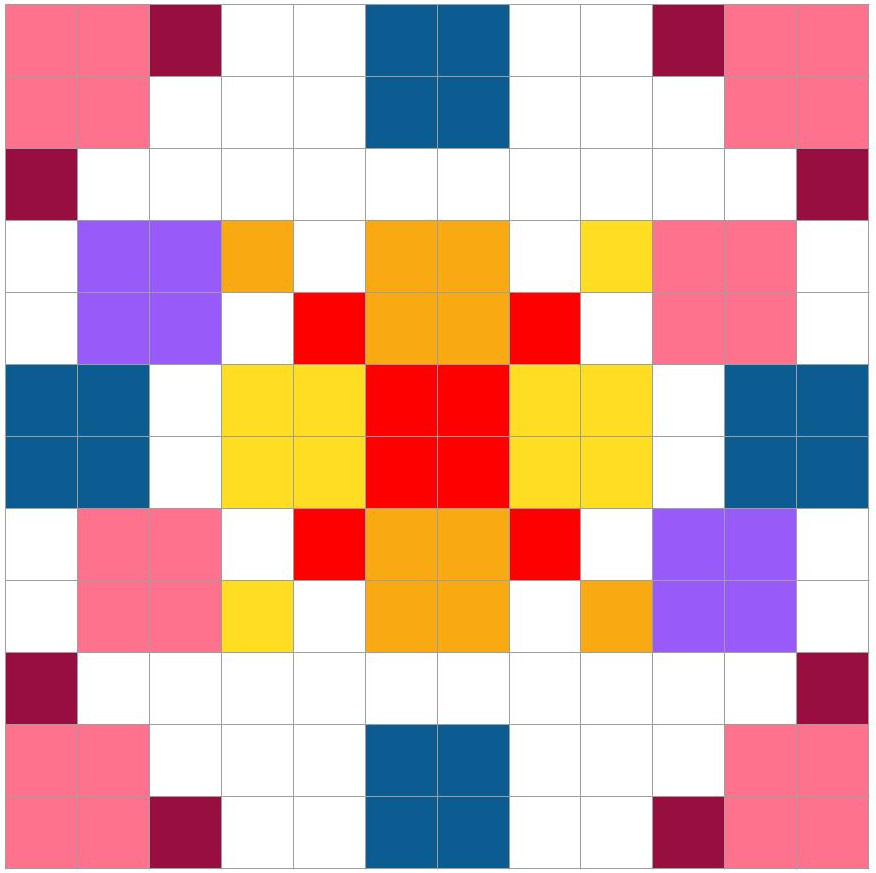
\includegraphics[scale=0.15]{First_ever.jpg}
\caption{Mosaic created with Beautiful Empathy}
\label{fig:mosaic}
\end{figure}

\lvl{}
\vspace{-1cm}

Beautiful Empathy is a collaborative board game in which players create a unique and colorful mosaic. The game has no scoring system and there is no official winner. The main outcome of the game is the mosaic built together. 

\lvl{Theme}

Lita loves art. She is happy when surrounded by beauty. For her house, Lita wants a mosaic full of colors unlike any before. To produce a completely original piece, she hires her favourite artists (the players) to paint in turns on a shared mosaic. Before a painting session, Lita spends some time with the painters, trying to understand them, to empathize with them. When Lita guesses the painter's minds, the artist becomes more productive and resourceful. By the end, all that matters is that the painters and Lita, are happy with the resulting artpiece.

\lvl{Game Script}

The game is played in six painting turns. On each turn, one player is the painter, who will \textit{feel} words in sentences, and paint on the mosaic. Another player is Lita, who tries to guess the painter's mind. Typically, roles will rotate among players, but well-intentioned alterations on who plays Lita are welcome. 

\lvl{The Empathy}

Each turn has two phases, the empathy and the beauty. In the first part, the empathy, Lita tries to figure out which word would the painter use to complete a sentence (out of two optional words). For example:

\begin{centering}
\texttt{Sentence:}\\
\textit{The tree was --------- in the middle of the forest}\\
\texttt{Options:}\\
\textit{shaking} | \textit{shinning}\\
\end{centering}
\vspace{0.5cm}

The painter must first read the sentence outloud with the two options, and quickly decide by instinct (and in silence) which one feels better. Lita must then guess which of the two options the painter chose. Empathy is key in this part.

After a round of 5 questions, and count the number of correct ones. More correct answers by Lita will better motivate the painter for the second part of the turn, the beauty. 


\lvl{The Beauty}

During this part, and in this order, the painter:
\begin{itemize}
 \item tries to \textit{add a new color} to it's palette
 \item draws cards to \textit{see the shapes available}
 \item \textit{place the tiles} on the mosaic
\end{itemize}

The painter can use any combination of colors in its palette when placing the tiles. Once all tiles have been placed, the turn is over and a new one can begin.

\sublvl{Add a New Color}

Each player starts the game with one random color. Or choose freely if you prefer. This is about having fun.

\begin{figure*}[th!]
\centering

\includegraphics[scale=0.6]{../boards/map_1.png}
\caption{Color map. There are 72 colors, starting on the center-left outside color (1 is the darkest pink, the clearest 61) and moving clock-wise. Each color is connected with the four colors that surround it. Border colors are also connected to all other border colors (outer among themselves and inners among themselves).}
\label{fig:color_map}
\end{figure*}

To gain a new color during your turn as a painter, first count the number of correct guesses from Lita. Then, if you have less than 4 colors, you get a new color. If you have 4 or more, and Lita did not guess a single word right, you get a color if you own less colors than correct guesses + 4. For example, a painter who owns 5 colors will get a new color if 2 or more questions were correctly answered by Lita. Five correct answers will always get the painter a new color, regardless of the colors already owned.

When adding a new color, the painter can choose from those directly connected to a color already owned. The colors each player owns are marked in the color map. Color can only be owned by a single player.


\sublvl{See Available Shapes}

After trying to get a color, the painter will find the material it has to work on the mosaic. This will depend on the palette and Litas empathy. A larger palette requires more paint, as more correct guesses motivate the painter to also paint more. In detail: 
\begin{itemize}
    \item \textbf{Palette size 1 to 3}:
    \begin{itemize}
        \item If Lita guesses 0 or 1, \\paint for 2 small squares (1x1)
        \item If Lita guesses 2 or 3, \\paint for 4 small squares (1x1)
        \item If Lita guesses 4 or 5, \\paint for 6 small squares (1x1)
    \end{itemize}
    \item \textbf{Palette size 4 to 6}
    \begin{itemize}
        \item If Lita guesses 0 or 1, \\paint for 8 small squares (1x1)
        \item If Lita guesses 2 or 3, \\paint for 4 small squares (1x1) \\and 2 big squares (2x2)
        \item If Lita guesses 4 or 5, \\paint for 8 small squares (1x1) \\and 2 big squares (2x2)
    \end{itemize}
    \item \textbf{Palette size 7 or more}
    \begin{itemize}
        \item If Lita guesses 0 or 1, \\paint for 4 small squares (1x1) \\and 2 big squares (2x2)
        \item If Lita guesses 2 or 3, \\paint for 8 small squares (1x1) \\and 2 big squares (2x2)
        \item If Lita guesses 4 or 5, \\paint for 16 small squares (1x1)
    \end{itemize}
\end{itemize}


\sublvl{Place the Tiles}

All that is left to do is for the painter to place the tiles on the mosaic. The painter has absolute freedom to do so, while the other painters can comment on the artistic aspects of it, before and after it is done. The placed tiles can be of any color available in the painter's pallette, and in any combination (different tiles, different colors). Try to respect the size of big squares, and the work of others.
% 
% \sublvl{Inspiration Bonus}
% 
% If Lita got 5 correct answers, the painter gains a bonus action, moved by her empathy. The painter draws from a uniform distribution of:
% \begin{itemize}
%     \item Choose and gift any color from the board to a fellow painter. 
%     \item Place 8 tiles on the mosaic with any colors of your choice (owned or not).
%     \item Change the color of 4 tiles already on the board to any of your choice (owned or not).
% \end{itemize}
% 
% 
At this point, this painter's turn is over. Call the next one in!

\lvl{End of Game}

The Game ends after six rounds. Or whenever you want. Once this is happens, take a look at the mosaic you created through empathy, and enjoy the beauty of your collaborative creation.

% \bibliographystyle{plain}
% \bibliography{references}
\end{document}
